\documentclass[12pt]{article}

\setlength{\textwidth}{17cm}
\setlength{\textheight}{24cm}
\setlength{\topmargin}{-2cm}
\setlength{\footskip}{1cm}
\setlength{\evensidemargin}{0cm}
\setlength{\oddsidemargin}{0cm}
\setlength{\parindent}{0cm}


\usepackage{amsmath}
\usepackage[magyar]{babel}
\usepackage[T1]{fontenc}
\usepackage[utf8]{inputenc}
\usepackage{fixltx2e}
\usepackage{multirow}
\usepackage{hyperref}
\usepackage{graphicx}
%\usepackage{gensymb}
\usepackage{float}

\begin{document}

%itt lesz a gorbe
A Lorentz-görbe a következő alakú:
\[  f(x) = \frac{a}{(1+s(x-x_0)^2)}\]
Ennek deriváltja
\[ \frac{df}{dx} = \frac{-2as(x-x_0)}{(1+s(x-x_0)^2)^2}\]

\begin{figure}[H]
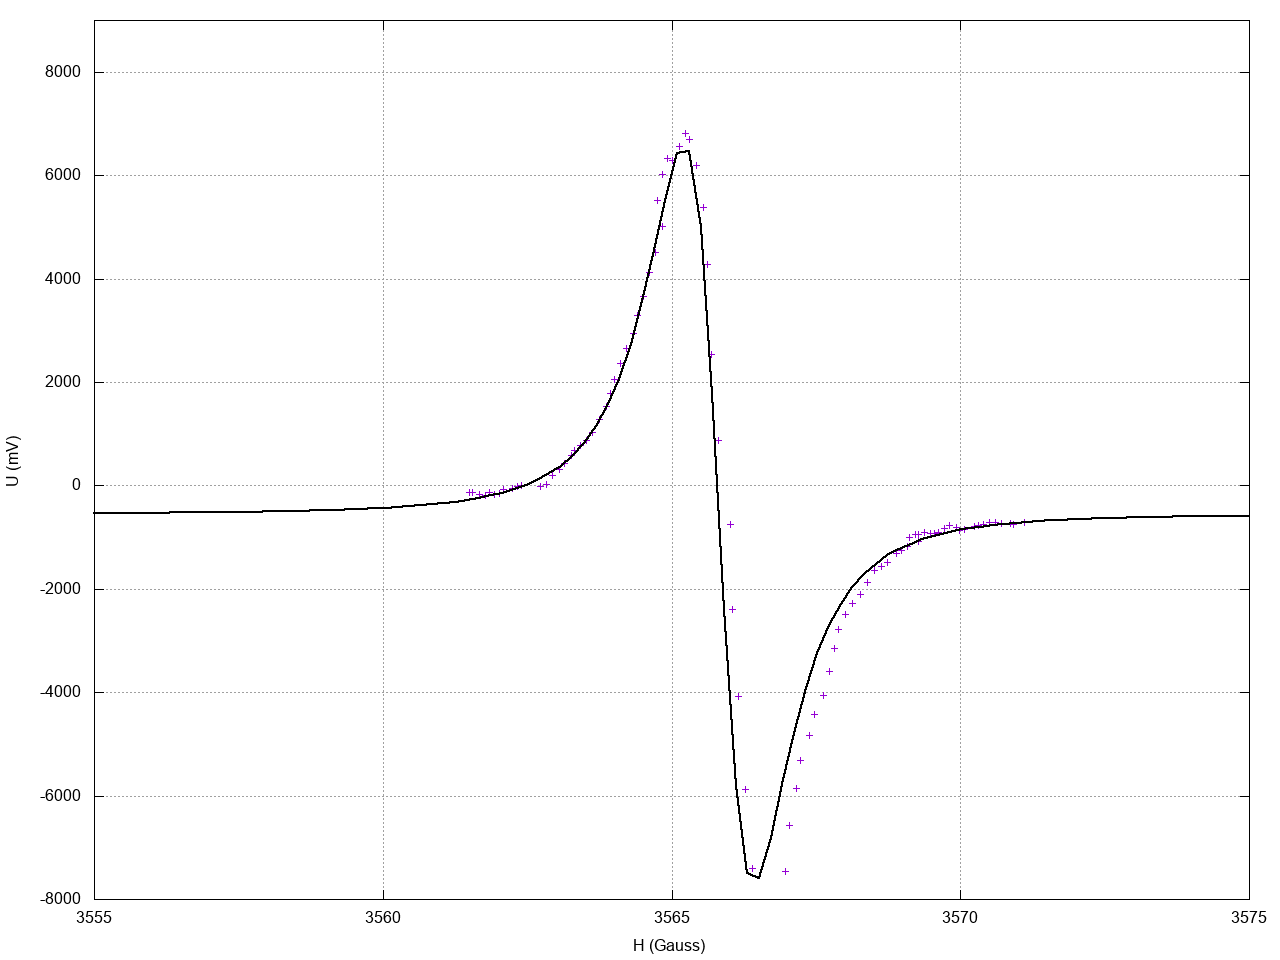
\includegraphics[width=15cm]{cr6.png}
\centering
\caption{A mérési adatok, és az illesztett derivált Lorentz-görbe Cr minta esetén}
\label{fig:3}
\end{figure}

\begin{figure}[H]
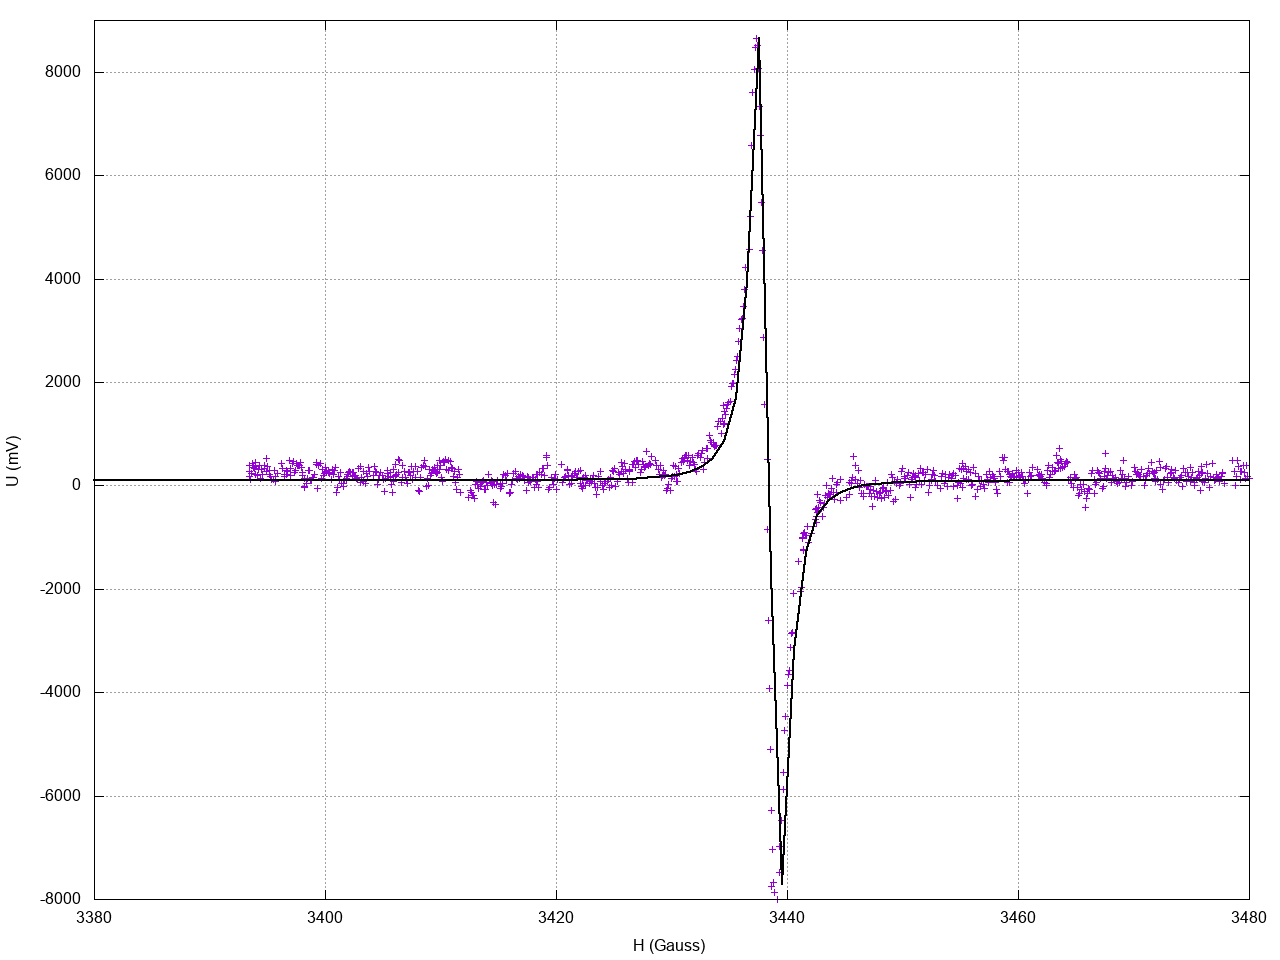
\includegraphics[width=15cm]{mn.png}
\centering
\caption{A mérési adatok, és az illesztett derivált Lorentz-görbe Mn minta esetén}
\label{fig:4}
\end{figure}

\begin{center}
\begin{table}[H]
\begin{tabular}{|c|c|c|c|c|c|c|c|c|}
 \hline
mérés & $a$ & $s$ & $x_0$ & $c$ \\ \hline
$1$ & $22977.3 \pm 1486$ & $1.030 \pm  0.099$ & $3224.82 \pm 0.1177$ & $-239.9 \pm 185.1$ \\ \hline
$2$ & $22630 \pm 890.9$ & $1.11 \pm 0.059$ & $3290.2 \pm 0.0855$ & $-300\pm 121.2 $ \\ \hline
$3$ & $20630 \pm 1267$ & $1.11 \pm 0.089$ & $3357.12 \pm  0.124$ & $-600 \pm 205.1$ \\ \hline
$4$ & $22570 \pm 789.7$ & $1.051 \pm 0.0512$ & $3425.36 \pm 0.0721$ & $-300\pm 127.1$ \\ \hline
$5$ & $22630 \pm 711.6$ & $1.0105 \pm 0.043$ & $3494.92 \pm 0.0662$ & $-204\pm 96.55$ \\ \hline
$6$ & $20524 \pm 1090$ & $1.2105 \pm 0.090$ & $3565.92 \pm 0.119$ & $ -700\pm 201.8$ \\ \hline
\end{tabular}
\caption{A $Mn$-minta esetében mért ESR jelre illesztett görbe paraméterei}
\label{tab:1}
\end{table}
\end{center}

Ezekből a számolt területek:
\begin{center}
\begin{table}[H]
\begin{tabular}{|c|c|}
 \hline
$\textrm{mérés}$ & $T$ \\ \hline
$1$ & $(7.1125 \pm 0.015)\cdot10^4$ \\ \hline
$2$ & $(6.7480 \pm 0.015)\cdot10^4$ \\ \hline
$3$ & $(6.1516 \pm 0.015)\cdot10^4$ \\ \hline
$4$ & $(6.9164 \pm 0.015)\cdot10^4$ \\ \hline
$5$ & $(7.0741 \pm 0.015)\cdot10^4$ \\ \hline
$6$ & $(5.8616 \pm 0.015)\cdot10^4$ \\ \hline
\end{tabular}
\caption{A $Cr$-minta esetében a Lorentz-görbe alatti területek}
\label{tab:2}
\end{table}
\end{center}


\begin{center}
\begin{table}[H]
\begin{tabular}{|c|c|c|c|c|c|c|c|}
 \hline
$a$ & $s$ & $x_0$ & $c$  & $T$ \\ \hline
$8524 \pm 223.7$ & $0.6105 \pm 0.02243$ & $3438.5 \pm 0.05018$ & $100 \pm 11.07$ & $(3.4287 \pm 0.015)\cdot10^4$ \\ \hline
\end{tabular}
\caption{A $Mn$-minta esetében mért ESR jelre illesztett görbe paraméterei}
\label{tab:3}
\end{table}
\end{center}

\end{document}
